%!TEX root = ../template.tex
%%%%%%%%%%%%%%%%%%%%%%%%%%%%%%%%%%%%%%%%%%%%%%%%%%%%%%%%%%%%%%%%%%%%
%% chapter2.tex
%% NOVA thesis document file
%%%%%%%%%%%%%%%%%%%%%%%%%%%%%%%%%%%%%%%%%%%%%%%%%%%%%%%%%%%%%%%%%%%%

\typeout{NT FILE chapter2.tex}%

\chapter{State Of Art}
\label{cha:Soa}

\glsresetall


\newpage
\section{Plantar Pressure Wearables}
\label{sec:plantar_pressure_wearables}

Plantar pressure wearables are innovative devices designed to monitor and analyze the distribution of pressure across the soles of the feet. By embedding sensors into insoles, smart 
socks, or even shoes, these wearables capture detailed data on foot loading patterns, which is critical for understanding gait, balance, and overall foot health. Plantar pressure data 
offers valuable insights for applications in sports performance, injury prevention, rehabilitation, and the management of conditions such as diabetes, where pressure distribution can 
indicate areas at risk for ulcers or other complications. They are also useful for better footwear designs or orthosis~\cite{coimbra, embedding, devInsole, deepLearn}.


As of today there are four different kinds of devices that can measure plantar pressure~\cite{smartSocks}:

\begin{enumerate}
  \item Platform Systems - Known as the most reliable method for measuring plantar pressure, platform systems offer high accuracy and detailed spatial resolution. Their main limitation is a lack of portability, restricting their use to controlled environments like labs and hospitals.
  \item In-Shoe Systems: These systems provide greater mobility and flexibility, with optimized circuit design, power efficiency, and communication technology, and they're more affordable than platform systems. They record plantar pressure inside the shoe and allow for extensive data collection across multiple steps, enabling long-term gait analysis indoors and outdoors. However, they are less accurate than platform-based measurements.
  \item Smart Wireless Insoles: Unlike platform and in-shoe systems, smart wireless insoles are cordless, eliminating the need for wires to connect sensors or data acquisition units. While in-shoe systems aren't ideal for extended outdoor use, smart insoles can be used both indoors and outdoors. They often include Bluetooth or WiFi for data transmission and a power source. However, the added elastic layer they create inside the shoe can be several millimeters thick, potentially distorting the accuracy of foot pressure data. They are also relatively expensive and not suited for daily wear.
  \item Smart Socks: These fabric-based systems integrate sensors directly into the textile, which avoids the challenges of the previous systems. However, they require handmade or complex manufacturing techniques, which is a drawback.
\end{enumerate}

In basketball, smart insoles and smart socks are particularly well-suited wearables due to their portability, flexibility, and adaptability to both indoor and outdoor environments. 
Unlike larger, stationary measurement systems, these wearable devices can move with the athlete, providing continuous and real-time data regardless of the set0ting.

Smart insoles, which are embedded with pressure sensors, can track a player's foot pressure distribution, stability, and impact forces with each step, jump, or landing. This information 
is crucial for basketball players, as it helps to analyze their movement patterns, improve balance, reduce injury risk, and enhance overall performance. The insole's thin profile and 
ability to fit inside regular shoes also ensure they don't interfere with the player's comfort or mobility.
Similarly, smart socks, which incorporate sensors directly into the fabric, offer flexibility and comfort while capturing dynamic foot pressure and movement data. Their lightweight 
design and close contact with the foot provide detailed insights into the nuances of foot pressure changes during the quick movements in basketball.
Both smart insoles and socks also benefit from wireless connectivity, allowing data to be transmitted to a smartphone or tablet, enabling real-time monitoring and analysis. This 
flexibility and data accessibility are particularly valuable in basketball training and performance analysis, as players and coaches can assess and adjust techniques in real time, 
whether in an indoor or outdoor court.


\subsection{Movement Recognition Wearables}
\label{ssec:movement_recognition_wearables}

As mentioned before in the introduction, there are many different wearables capable of collecting the same type of data but in different ways. %, devInsole
For gait monotoring there are several different types of sensors used in wearables that can be separated in five different categories~\cite{smartSocks}:


\begin{enumerate}
  \item Capacitive Sensors - Consisting in two conductive plates separated by an insulating layer. When force is applied, they develop a voltage variation.
  \item Resistive Sensors - These are the most common sensors. Their resistance varies with the applied pressure.
  \item Optoelectronic Sensors - Composed by a trasmitter and a receiver (a laser or a LED and a photodiode). When a force is applied, the light that reaches the photodiode varies proportionally.
  \item Piezoresistive and Piezoelectric Sensors - These sensors use the  piezoelectric effect. They convert the changes in applied pressure to eletrical corrent.
\end{enumerate}

%Muscle Sensors
\subsection{Restraints}
\label{ssec:restraints}

Wearables have to be light and comfortable since they should be unnoticeable and not disturb the user's activities. This means that these gadgets have low processing capacities 
and their sensors monitor the data at lower frequencies then non wearable devices. Due to their size they often use miniature sensors that can be sensitive to placement and alignment. 
Inaccurate placement, external interference, or device movement can cause errors, reducing the reliability of collected data. Additionally, in applications where precise measurements 
are essential, the smaller sensors in wearables can't match the accuracy of larger, lab-based equipment.

Wearables are often exposed to a wide range of environmental conditions, including sweat, water, dust, and physical impacts. Ensuring these devices remain durable and function properly 
under such conditions is a challenge, as components like sensors and circuits need to be robust enough to withstand daily use and environmental exposure.

Due to their lack of memory and processing power, the data collected from the devices has to be sent to another device for storage or further processing. The main communication protocols 
with low energy consumption are Bluetooth Low Energy (BLE) and WiFi for close data transmission. These methods can be impacted by limited range, interference, and connectivity issues, 
especially in crowded or signal-dense environments, which can disrupt real-time data streaming.

Since these devices are quite small, one of their main restraints is the battery life. With every action taken by the device, wheter it's collecting data with a sensor, processing that data or sending it 
somewhere else, energy is always spent. Depending on their purpose, wearables may have to last up until one year without being charged~\cite{challengesWearables}. To overcome this challenge 
some devices rely on energy harvesting components to charge the device such as solar power, motion energy, etc~\cite{embedding}.

Minding the others problems already mentioned, wearables have low security so they are relatively easy targets due to their poor encryption and protection~\cite{wearablesAndIOT}.
Due to the lack of privacy of the athlete's data and since wearable technology can possibly obstruct and injury someone, wearables still are'nt accepted in many sports 
(in federated play), basketball included. Even tho they are't allowed in games, there aren't any rules for practices and there are some teams that are taking advantage of these 
devices~\cite{NBPAWearables, hawksWear}.


\subsection{Communication Protocols} %dá para aumentar
\label{ssec:communication_protocols}

Wearable technology relies heavily on efficient communication protocols to ensure seamless data exchange between devices, applications, and networks. These protocols define the rules 
for data transmission, enabling wearables to monitor health, track activity, and connect with other devices in real time. Given the constraints of wearables, communication protocols 
play a critical role in balancing performance with power efficiency.
For this project two kinds of protocols will be discussed: Bluetooth Low Energy and WiFi.


\subsubsection{Bluetooth Low Energy (BLE)}
\label{sssec:ble}

Bluetooth Low Energy (BLE) is a short-range communication technology known for its low power consumption. Classified as a Wireless Personal Area Network (WPAN), BLE is widely used in 
various wearable applications, from diabetes monitoring devices to smartwatches. The original insole design employed BLE for communication between the insole and the paired mobile application.
BLE's primary design objectives are to enable low-power communication, particularly for peripheral devices. It is optimized for affordability and simplicity, aligning well with many 
developer requirements and contributing to its swift adoption.
The main difference between BLE and the classic Bluetooth is their transmition rates. BLE transmits at around 2000 Kbps while Bluetooth Classic transmits at around 2-3 Mbps making its energy comsuption 
around two times bigger than BLE. This is the reason BLE is the usual choice for IOT devices. Besides this difference BLE works the same way as Bluetooth Classic~\cite{masterInsole, bachelorInsole}.

\subsubsection{WiFI}
\label{sssec:wifi}

WiFi is a widely used wireless Local Area Network (LAN) technology, primarily aimed at connecting mobile devices to the internet. Its broad adoption means it's available in most homes, businesses, and many public 
spaces. WiFi uses variations of the IEEE 802.11 protocol depending on the generation, with the latest generation, WiFi 6 (802.11ax), approved in September 2024. Operating on the 2.4 GHz or 5 GHz 
frequency bands, WiFi 6 also supports wider channels, optimized mainly for video streaming.
WiFi delivers high data speeds and easy setup for access points, making it a mature and well-proven technology. However, its range is somewhat limited indoors due to high signal 
absorption, though range improves in open, line-of-sight environments. Due to its relatively high power consumption, WiFi is not ideal for direct communication in IoT devices~\cite{masterInsole, bachelorInsole}.

\subsection{Gait Cycle}
\label{ssec:gait_cycle}

The Gait Cycle is the sequence of movements that one leg takes in each step in walking or running. It is the whole moving process from the first point of contact between 
a foot and the ground until it reaches the ground again (see figure\ref{fig:gaitCycle})~\cite{masterInsole, freewalker}.

\vspace{.5cm}
\begin{figure}[htbp]
    \centering
    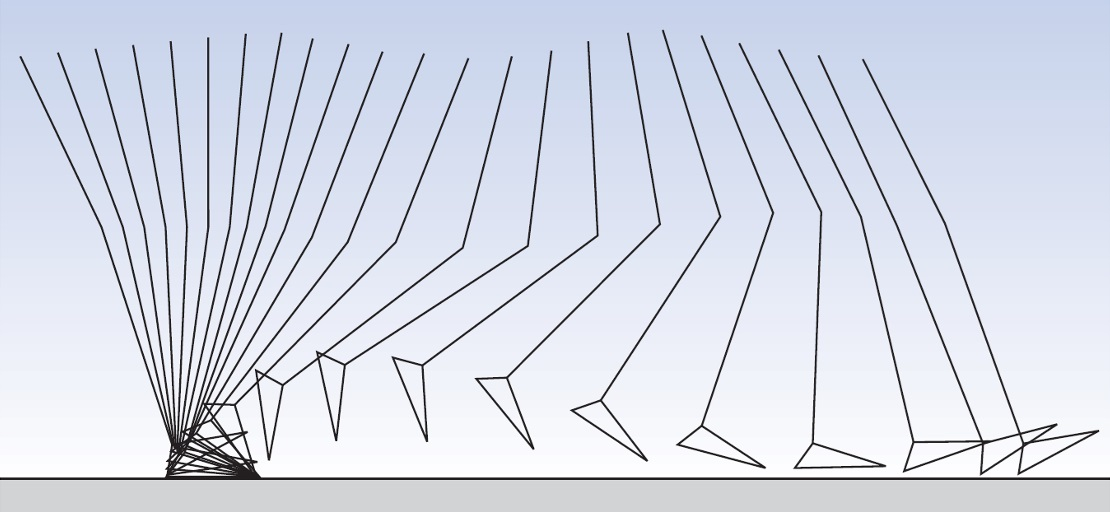
\includegraphics[width=0.8\linewidth]{gaitCycle.jpg}
    \caption{The gait cycle of a leg with with a cycle time of 0.92s. 40 ms interval between lines~\cite{gaitBook}.}
    \label{fig:gaitCycle}
\end{figure}

The usual method for measuring Gait Cycle is with a platform and a multi-camera setup since it is the most precise and reliable. However, this method is very expensive and can only be 
applicable indoors in a secure environment. An insole or a smart sock aren't as reliable but they compensate by being cheaper, more comfortable for the user and can be worn in their activities.

Although the Gait Cycle varies from person to person (minding age, body type and others) and even in each step each person takes, there are many tendencies for normal gait.
With this in mind these patterns can be used to predict and understand what forces are applied in a gait cycle~\cite{masterInsole}.

There are three foot's directions(see figure\ref{fig:footDir}): Vertical which is the direction perpendicular to the foot's palm. Fore-aft that follows the line between the toe to the heel. And the 
lateral direction which goes from one side of the foot to the other~\cite{masterInsole}.

\begin{figure}[htbp]
  \centering
  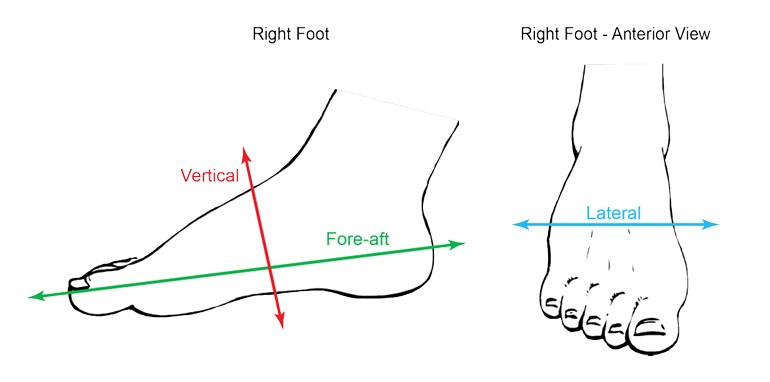
\includegraphics[width=0.7\linewidth]{footDir.jpg}
  \caption{The three foot's directions~\cite{gaitBook}.}
  \label{fig:footDir}
\end{figure}


There are two different stages for this motion in slower gaits and an extra stage in faster gaits~\cite{porto}:

\begin{itemize}
  \item Stance Phase - when the foot is in contact with the ground. This represents about 60\% of the normal gait cycle.
  \item Swing Phase - when the foot is in the air. It normally represents the remaining 40\% of the gait cycle.
  \item Flight Phase - this phase only occurs in faster gaits such as running. It refers to the moments where neither foot is in contact with the ground.
\end{itemize}

\newpage

\subsection{Other Movements}
\label{ssec:other_movements}

Basketball involves many other distinct movements besides gait. These motions are very complex making them difficult to accurately identify 
but they are essencial for injury prevention and for the perfomance enhancement analysis. In this project data will be collected from three groups of movements with increasing complexity.

\begin{figure}[htbp]
  \centering
  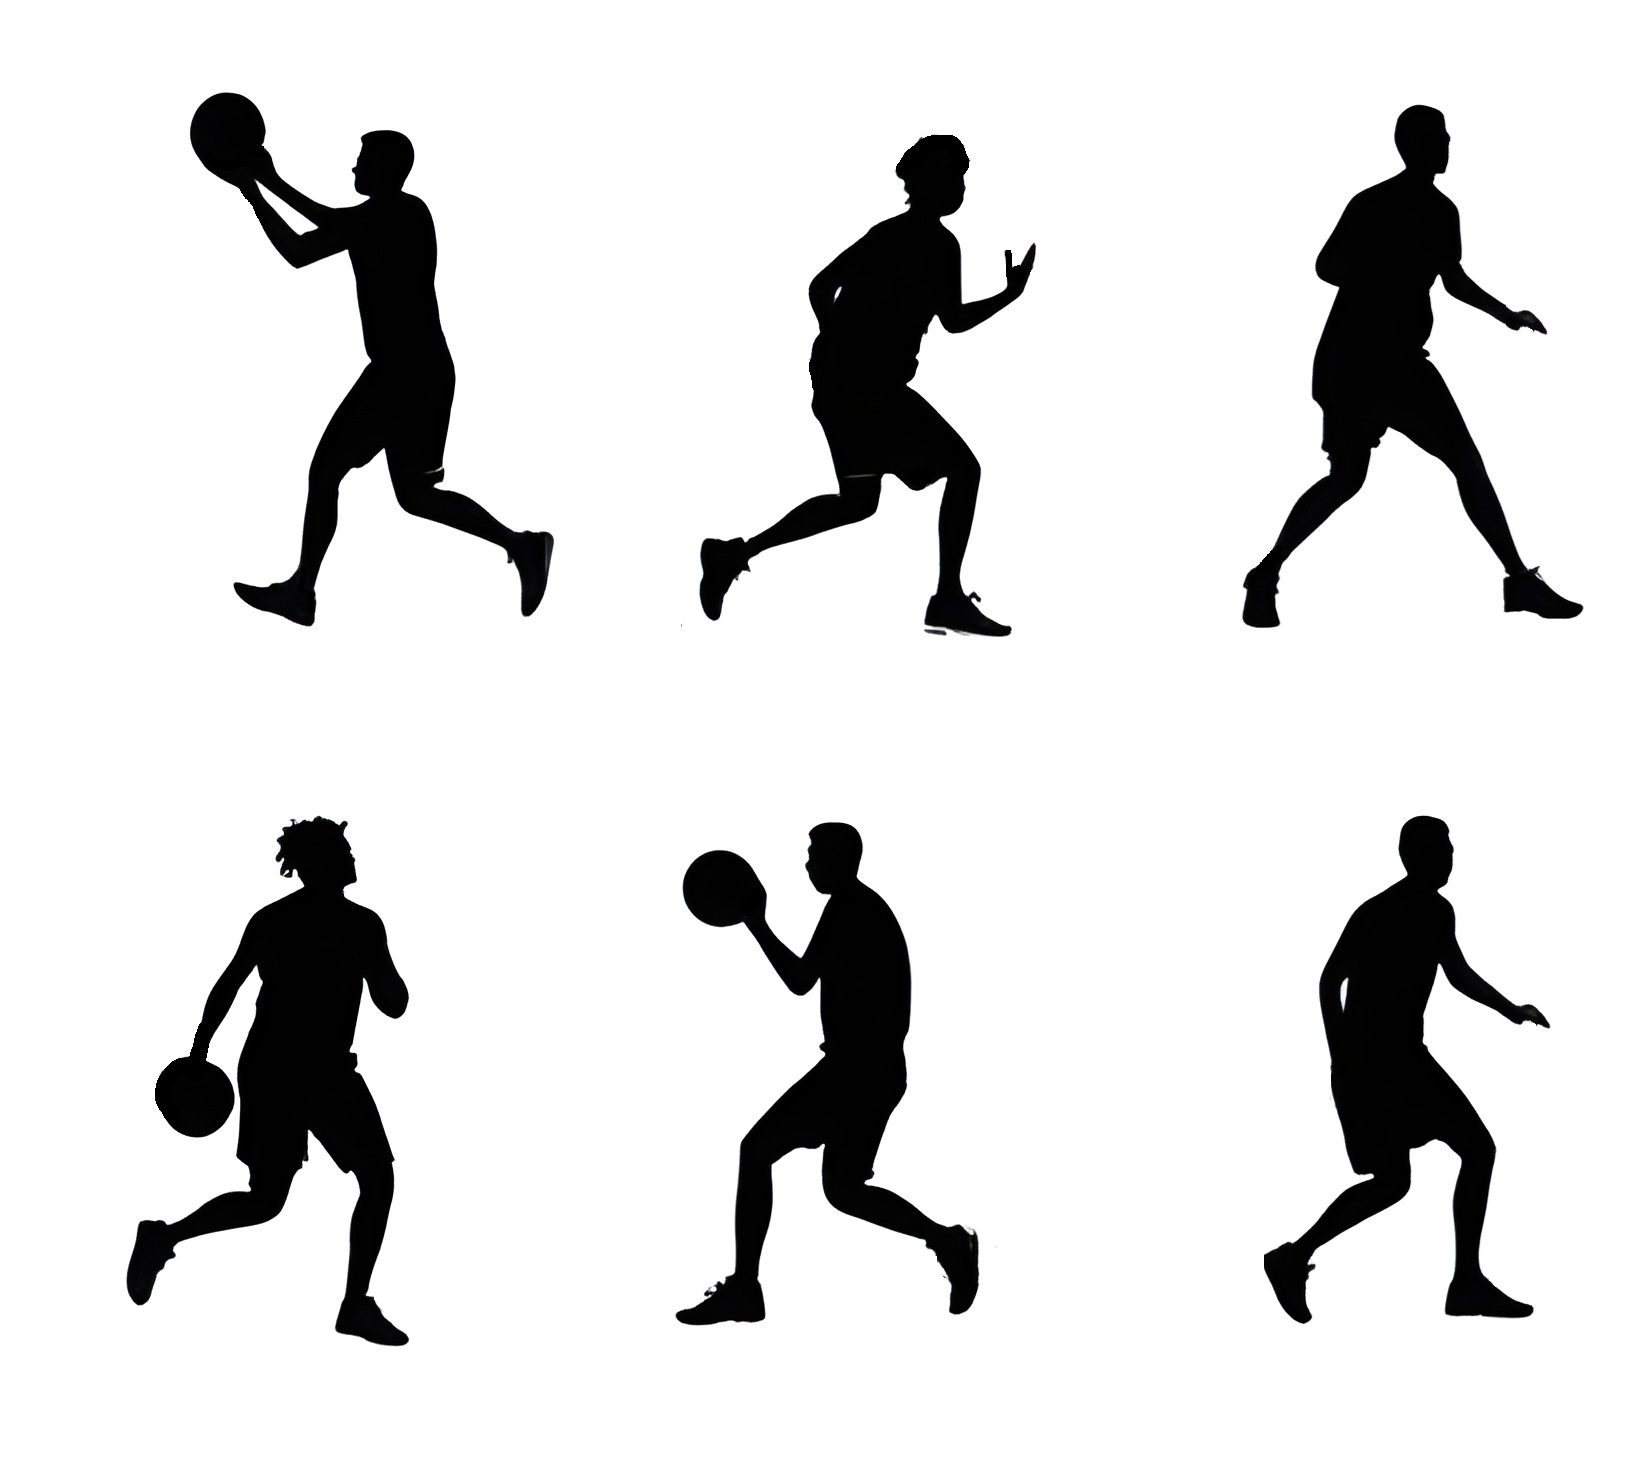
\includegraphics[width=0.6\linewidth]{basketPos.jpg}
  \caption{Some basketball stances.}
  \label{fig:basketPos}
\end{figure}

\subsubsection{Basic Movements}
\label{sssec:basic_movements}

\begin{itemize}
  \item Layup - A layup is normally a two step shot and it requires a step-by-step increase in pressure, usually peaking in the final step before jumping.
  \item Crossover Dribble - In a crossover dribble, the player shifts their weight rapidly from one foot to the other, using pressure changes to decelerate in one direction and quickly accelerate in the opposite direction.
  \item Sprint(fast gait) - Basketball players frequently sprint down the court, which involves a pattern of quick, alternating footfalls with consistent gait cycles on each foot.
  \item Defense Slide/Stance - The defensive slide requires the player to move laterally while maintaining a low stance.
  \item Boxout - The act of securing a positing usually near the basket to deny the rebound for the opponent.
  \item Rebound Jump - Rebounding requires explosive jumping to reach the ball, sometimes with minimal preparatory movement, other times with a box out.
  \item Cutting - Cutting involves a sharp change in direction with a great speed shift. It is an offball movement.
  
\end{itemize}

\subsubsection{Intermediate Movements}
\label{sssec:intermediate_movements}

\begin{itemize}
  \item Pivot - A pivot involves planting one foot firmly while the other foot moves to change direction.
  \item Change of Direction in Defense - A player changes his direction while sliding.
  \item Screen - Similar to the boxout but it is done anywhere on the court to force a defensive player to change his path.
  \item Jumpshot - The act of shooting the ball. The jump shot is a fundamental shooting technique in basketball, characterized by a quick dip in pressure as the player lowers into a squat before takeoff, followed by a burst of force as they push off the ground to jump.
\end{itemize}

\subsubsection{Advanced Movements}
\label{sssec:advanced_movements}

\begin{itemize}
  \item Eurostep - This movement is a specific type of layup where the player takes the first step in a direction and the second step to another direction.
  \item Step Back - The step back is a Jump Shot whe the player takes a step back before shooting the ball.
  \item Failed Landing (Incomplete layup) - Any type of fall characterized by the sudden fall of pressure and followingj.

\end{itemize}

\newpage
\section{Related Work}
\label{sec:related_work}

There are many studies on the topic of measuring plantar pressure through an insole. Most of them mostly study the gait cycle while running or walking with similar objectives. 
Baitong Wang et al.~\cite{freewalker} developed an insole with 8 pressure sensors and motion track sensors and with this system managed to clearly identify gait with only the pressure 
sensors.

Elizabeth S. Chumanov et al.~\cite{posDuringWalking} tracked the global position of the pressure on the soles of the feet throughout steps in walking and running. This data can be used 
for improvement in foot-floor contact models used to simulate human locomotion and in least squares inverse dynamics.


For sports like basketball, the available motion recognition research was done through video recording or smart wearable devices such has wristbands. There is very few studies on the 
use of insoles for this purpose. 

Thomas Holleczek et al.~\cite{snowboard} design a pair of smart socks with three pressure sensors each for the use case of snowboard. Even tho it isn't a sport as dynamic and unpredictable 
as basketball, it still is very relevant for this project. They worked on activity recognition focusing on recognizing if the user was riding backside or riding frontside (with his 
back to the bottom of the hill or the top respectively). It is pointed that the recognizability of three basic standing postures was explored and that they were distinguished with perfect accuracy 
mentioning that it can be interesting for gait analysis.


Qing F. Zhou et al.~\cite{basketballMotions} utilized insoles with a motion sensor with the purpose of getting a high accuracy for recognizing three basketball motions: 
Dribbling, jumping and turning around. For this data processing the K-means algorithm was utilized. 
Two years later they continued their work and managed to identify five new different 
footwork movements. In this version a multiple sensor system was proposed and three different classification methods were discussed~\cite{basketballFootwork}:
K-Nearest neighbours (KNN), Support vector machine (SVM) and Convolutional Neural Networks (CNN).


Catarina Amaro et al.~\cite{coimbra} studied the differences in five different movements in basketball between two different moments in a season. The study presented no significant 
changes in mean peak pressure between the two different times but it did specify that experienced players had lower plantar pressure values in their movements and lower symmetry index. This means that there 
is room for improvement based on the values read for the less experienced players. It was also mentioned that wear of the shoes may have influeced the slight changes observed in the study. 
Each player weared their own shoes and this was pointed as a variable for the plantar pressure measured.

\newpage

\section{Relevant data for analysis}
\label{sec:relevant_data_for_analysis}

Wearable devices capture large volumes of raw data, often gathering detailed metrics like pressure distribution, movement patterns, and force dynamics. However, to extract meaningful 
insights, this raw data must first be transformed into a more organized, manageable format suited for analysis. Preprocessing includes filtering out noise, aligning data with relevant 
time frames, and structuring it into clear categories or features, which simplifies identifying trends and patterns. By converting this data into a cleaner, standardized format, we can 
more effectively apply analysis techniques, uncovering insights into biomechanics, performance, and even long-term health outcomes.

%\subsection{Center of Mass (COM) and Center of Force (COF)}
%\label{ssec:com_and_cof}

%The COM is the average position of a any mass, which means that if you were to balance the system at this point, it would be stable and balanced. The exact location of the COM in a 
%human body varies depending on posture, position, and body type but is generally around the pelvis when standing upright. For a group of identities it can be calculated by the following 
%equation\cite{masterInsole}:

%\[ COM = \frac{m_1 \cdot x_1 + m_2 \cdot x_2 + m_x \cdot x_x}{m_total} \]

%The center of force (COF) is the point where the total force exerted on a surface, such as the ground or a support, is concentrated. In biomechanics, especially in gait and balance 
%studies, the COF reflects the point where all pressure forces on the foot combine during contact with the ground. Unlike the center of mass (COM), which relates to the body's weight 
%distribution, the COF is influenced by how the body applies force through specific contact points (like the heels or balls of the feet) while standing, walking, or running.
%For example, when a person shifts weight from one foot to the other, the COF moves in response to this change in pressure. During a step, the COF generally shifts from the heel at 
%initial contact toward the toes before push-off, tracking the path of weight transfer. 


\subsection{Average Pressure}
\label{ssec:average_pressure}

Foot therapists currently rely on average pressure to determine if a support sole is effective and where additional relief might be needed. This average provides an interpretable view 
of pressure distribution during the gait cycle. However, averaging all values across all frames would dilute important information because of the many zero values present throughout 
the cycle. To avoid this, only non-zero values are averaged for each sensor. Yet, this approach introduces another challenge: a cell with few non-zero readings could appear similar to 
one with many readings. To improve clarity, cells are excluded from analysis if they don't exceed a minimum threshold of non-zero measurements for that sensor\cite{masterInsole}.


\subsection{Peak Pressure (PP), Pressure Time Integral (PTI) and Mean Peak Pressure (mPP)}
\label{ssec:pp_pti_mPP}

When assessing plantar pressure, the primary parameters of interest are peak pressure (the highest recorded plantar pressure), pressure time integral (typically defined as the 
area beneath the peak pressure-time curve), and mean peak pressure (mPP). However, studies have shown that mPP and PTI are closely related, making it unnecessary to measure both.

When there are diferences in these measurements between the feet, it can mean that there is an inadequate distribution of forces and it can lead to injury. So a symmetry index defined by 
the next equation that compares the plantar pressure on both feet will be calculated.

\[ SI = \frac{2 \cdot \left\lvert R - L\right\rvert }{(R + L)} \times 100 \]

If SI is zero then the feet are doing equal work, if it's under 10\% it is acceptable, otherwise it means the movement is causing more distress in one leg than the other leading to a 
loss of bone mass density in the respective leg and joints~\cite{coimbra}.


\newpage
\section{Data Analysis}
\label{sec:data_analysis}

By leveraging advanced data analysis techniques, such as machine learning algorithms and statistical modeling, pressure insole data can reveal subtle patterns and correlations that 
inform training adjustments, injury risk, and performance improvements. There are many different algorithms with different objectives. In this section some of them will be explained:


\subsection{K-nearest-neighbours classfication}
\label{ssec:k-nearest_neighbours}

The K-nearest-neighbours is one of the simplest supervised machine learning algorithms. It's a classification algorithm which uses proximity to assigning each point to the class with 
the most similar elements within the K-nearest-neighbours~\cite{bachelorInsole, porto}. 

As an example observe figure\ref{fig:k-near}. If someone would have to assign a class (green diamonds, blue squares or red circles) to the cross in the figure, they would probably say it belongs to the green diamonds since 
they are the closest objects. But if instead someone had to assign a class for the star, it would be a much harder task with a naked eye. 
In this case two factors make that decision: Which are the closest objects (depending on the weight k) and how many of each class are there in that group~\cite{bachelorInsole}. In other words 
imagine a small circle with its center on the object that we want to classify and if it isn't touching other know objects imagine it growing until it does.

\begin{figure}[htbp]
  \centering
  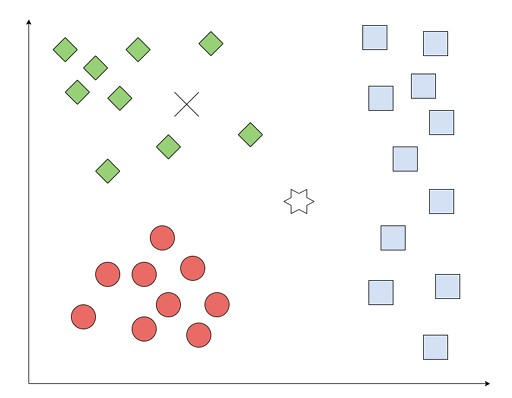
\includegraphics[width=.5\linewidth]{k-near.jpg}
  \caption{K-nearest-neighbours example~\cite{bachelorInsole}}
  \label{fig:k-near}
\end{figure}

\subsection{Dynamic Time Warping}
\label{ssec:dynamic_time_warping}

The dynamic Time Warping (DTW) algorithm transforms unsynchronized time series or time series with different lengths allowing a dynamic comparison between them. This algorithm calculates 
the best possible alignment between two different series dependent on time providing a measurement of how well aligned (or not) they are~\cite{bachelorInsole}.

\subsection{Regression analysis}

Regression analysis' purpose is to find a continuous outcome variable, usually y, through one or more predictor variables, normally x (if only one). The simplest of these models is the 
linear regression model that relates a linear relationship between x and y. This equation can be expressed as~\cite{bachelorInsole}:
\[ y = \beta + \alpha \cdot x + \epsilon \]

In this equation y is the output variable, $\beta$ is the starting point (x=0), $\alpha$ is the regression coeficient associated with the predictor variable x and $\epsilon$ is the residual error.
An extended version of this equation with n predictor variables is:
\[ y = \beta + \alpha_1 \cdot x_1 + \alpha_2 \cdot x_2 + \alpha_n \cdot x_n + \epsilon \]

\subsection{Recursive Feature Elimination}
\label{ssec:recursive_feature_elimination}

Recursive Feature Elimination (RFE) selects features by progressively narrowing down the set of available features. Each feature is assigned a weight, and those with the lowest absolute 
weights are removed from the set. In each iteration, a single feature is removed, and this process continues on the reduced set until the target number of features is reached~\cite{porto}.


\subsection{Principal Component Analysis}
\label{ssec:principal_component_analysis}

Principal Component Analysis (PCA) reduces the dimensionality of data by applying a linear transformation based on singular value decomposition. This transformation projects the data 
into a lower-dimensional space, creating a new set of variables that are ordered by their importance~\cite{porto}.


\subsection{Linear Discriminant Analysis}
\label{ssec:linear_discriminant_analysis}

The Linear Discriminant Analysis (LDA) model fits a Gaussian distribution to each class, assuming a shared covariance matrix across all classes. This model reduces input dimensionality 
by projecting data onto the directions that best separate the classes. Its goal is to enhance separation between classes by maximizing the scatter between them while minimizing scatter 
within each class~\cite{porto}.


% \printbibliography[heading=subbibliography, segment=\therefsegment, title={\bibname\ for chapter~\thechapter}]
